
%Emergency service systems: 
%The use of the hypercube queueing model in the solution of probabilistic location problems

\section{Hypercube queening model}
\subsection{Introduction}
\begin{frame}
  Given a system configuration, 
the hypercube model is able to evaluate a variety of performance
measures relevant for decision-making, 
either region-wide or for each server or region.

These include 
server workloads, 
mean user response times, 
fraction of dispatches of each server to each region,
among others.
\end{frame}

\begin{center}
  % Pendiente, ajustas coordenadas
  \begin{tikzpicture}
    \node[anchor=south west,inner sep=0] at (0,0) {
      %\includegraphics[width=0.9\textwidth]{tmax}
      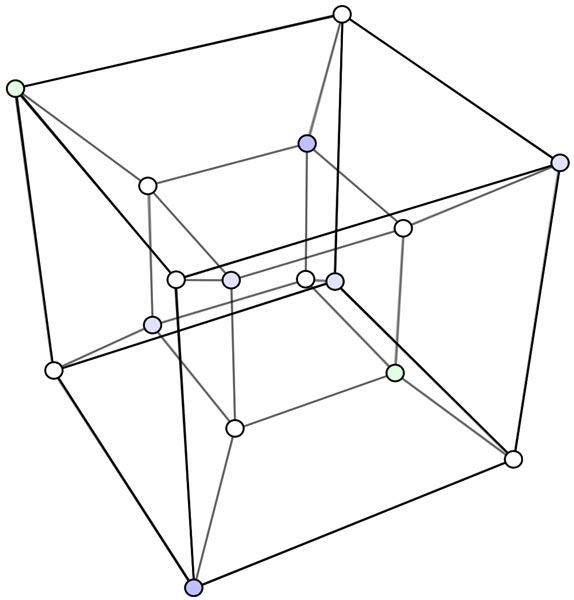
\includegraphics[scale=0.3]{hypercube}
    };
    \draw (2.5,0.1) node {\scalebox{.4}{(0,0,0,0)} };
    \draw (5.9,1.5) node {\scalebox{.4}{(0,0,0,1)} };
    \draw (2.9,1.8) node {\scalebox{.4}{(0,0,1,0)} };
    \draw (1,2.4) node {\scalebox{.4}{(0,1,0,0)} };
    \draw (2.2,3.65) node {\scalebox{.4}{(1,0,0,0)} };
  \end{tikzpicture}
\end{center}
\end{frame}

\subsection{Basic assumptions}
\begin{frame}{Geographical atoms and arrival processes}
  \begin{enumerate}
  \item The region is divided into \textit{M} geographical atoms,
    which correspond to non-overlapping areas of a city
  \item The emergency calls of each atom \textit{j} occur as a Poisson
    process, independently from the other atoms, with mean arrival rate $\lambda_j$
  \item The mean travel times $\tau_{ij}$ between atoms are known
  \end{enumerate}
\end{frame}

\begin{frame}{Servers and service processes}
  \begin{enumerate}
  \item There are \textit{N} spatially distributed servers, 
    which can service any atom
  \item Each server, when idle, stays in its base waiting for a call, 
    or moves inside a determined area
  \item The service time for a call includes the set-up time, 
    the travel time from the base until the location of the accident, 
    the on-scene time, a possibly related follow-up time, 
    and the travel time back to the base
  \item Variations in the service time that are due to variations in travel time 
    are assumed to be of second order when compared with variations of set-up, 
    on-scene and related follow-up times
  \end{enumerate}
\end{frame}

\begin{frame}{Server assignment and fixed-preference dispatching}
  \begin{enumerate}
  \item In response to each call, 
    exactly one server is dispatched from its base to the location of the accident
  \item If there are no available servers, 
    the call is either queued and serviced according to an FCFS discipline,
    or it is lost
  \item There is a list of dispatching preferences for each atom
  \end{enumerate}
\end{frame}

\subsection{Calibration process of the mean service times}
\begin{frame}
In this emergency system, 
travel times may represent a considerable part of service times. 
It may be advisable to adjust the service times by means of a calibration process,
which can be performed using a simple iterative procedure.

The procedure consists of 
verifying if there are significant differences among 
the input mean service times and the output mean service times (computed by the hypercube model). 
In this case, 
the hypercube is solved using the computed mean service times as inputs, 
until the differences among input and output values are sufficiently small
\end{frame}

\begin{frame}{}{}
  {\footnotesize
  \begin{center}
    The mean service time calibration method
  \end{center}
  \vspace{-8pt}
  \hline \\
  \vspace{2pt}
  \textit{Step 0.} The mean service time of unit \textit{i},
  $1/\mu^{i}=1/\mu_{NT}^{i}$, $i = 1,\ldots,p$ 
  ($1/\mu_{NT}^{i} = \sum_{j=1}^{n}{h_j\bar{W_{ij}}}$ 
  is the mean of non-travel time component of the service time). \\
  \textit{Step 1.} Run the Hypercube Model (using $\mu^i$) to obtain $f_{ij}$, $i = 1,\ldots,p$, $j = 1,\ldots,n$. \\
  \textit{Step 2.} $1/\hat{\mu}^{i} = \sum_{k=1}^{n}{h_{k}^{i}(\bar{W_{ik}}+(\beta_{i}/v_{i})d_{ik})}$ where $h_{k}^{i} = f_{ik}/\sum_{j=1}^{n}{f_{ij}}$ \\
  \textit{Step 3.} If $|1/\hat{\mu}^{i}-1/\mu^{i}|>\epsilon$ for at least one $i$, $i=1,\ldots,p$, set $1/\mu^{i} \equiv 1/\hat{\mu}^{i}$ and go back to \textit{Step 1.} Otherwise stop. \\
  \hline
}
\end{frame}
